% latexmk -pvc -pdf
\documentclass[9pt, a4paper]{article}
\usepackage[margin=0.65in]{geometry}
\usepackage{graphicx}
\usepackage{caption}
\usepackage{amsmath,amsthm,amsfonts,amssymb}
\usepackage{blindtext}
\usepackage[english]{babel}
\newenvironment{Figure}
    {\par\medskip\noindent\minipage{\linewidth}}
    {\endminipage\par\medskip}

% \newcommand\II{\mathbb{}}
% \newcommand\PT{\textit{}}

\title{Simulating phase contrast imaging for materials with variable density (PART II)}
\author{Ana C. Fabela Hinojosa \\
\small{Supervisors: Assoc. Prof. Marcus Kitchen}}
\small{\date{\today,  \\Due date: Friday 26\textsuperscript{th} August, 2021}}

\begin{document}
\maketitle
\section{Current objective}
% In this project I study the theoretical perspective of coherent X-ray imaging. My current focus is to investigate via a simulation how the phase of incident X-rays changes as the density of a sample material in an arbitrary imaging system changes. My investigation will be extended by simulating two distinct materials under the same wave-field and see if and how distinctly phase contrast occurs. The eventual goal of this simulation is to verify if successful phase retrieval can be done of the imaged objects given their variable densities.

\section{Computational fundamentals}


\section{Investigations}
% The simulation that I am presently working on involves a cylinder made of a single material (i.e. monomorphic) with constant density. My supervisor and I are curious to see if we can verify a claim in one of the texts I am using in my research. This claim concerns a propagation based phase contrast imaging (PBI) algorithm that was first developed by Paganin et al. (2002)\cite{Pags2002}\cite{CH49}. Specifically, the claim states that the stability of Paganin's algorithm is thought to be dependent among other factors in the ratio between $\delta$ and $\mu$, both of which are proportional to the density of the medium. The conclusion from this claim is essentially that: any changes in material density throughout the material would not affect the imaging process. My supervisor suspects that this statement might not be entirely correct and we want to verify if the stability of the Paganin et al. (2002) algorithm is dependent instead on the ratio of the differences in the refraction and attenuation coefficients $\Delta \delta$ and $\Delta \mu$.

\subsubsection{Current progress}
% I am inspiring some of my work in a paper by Beltran et al. (2010) (see reference \cite{Beltran}), their approach requires just a single phase-contrast projection, and enables the user to focus on a material of interest. In the case of my simulation, I set the complex refractive index, and thickness of the imaged cylinder based on the parameters given in Beltran et al.(2010)\cite{CH49}. For simplicity, my supervisor and I decided that I should break my simulation into simpler tasks. Therefore my first simulation will be that of a single monomorphic cylinder, and later on I will work on 2 cylinders, one embedded on another, both these cylinders will have different densities, since I want to understand how much density difference is needed before I see phase contrast in my simulation.
% To solve the transport-of-intensity equation (TIE) and go beyond the projection approximation I have designed a differential equation solver using the fourth order Runge-Kutta algorithm. Since there is an intrinsic link between the phase and the TIE, I decided to solve re-write equation (\ref{eq:15}) in differential form and solve it simultaneously to the TIE in my code.
% So far I have been able to recover the phase gained by the incident X-ray wave-fronts as they cross the cylindrical material I simulated.
% \subsubsection{Results}
% \begin{Figure}
% \centering
% 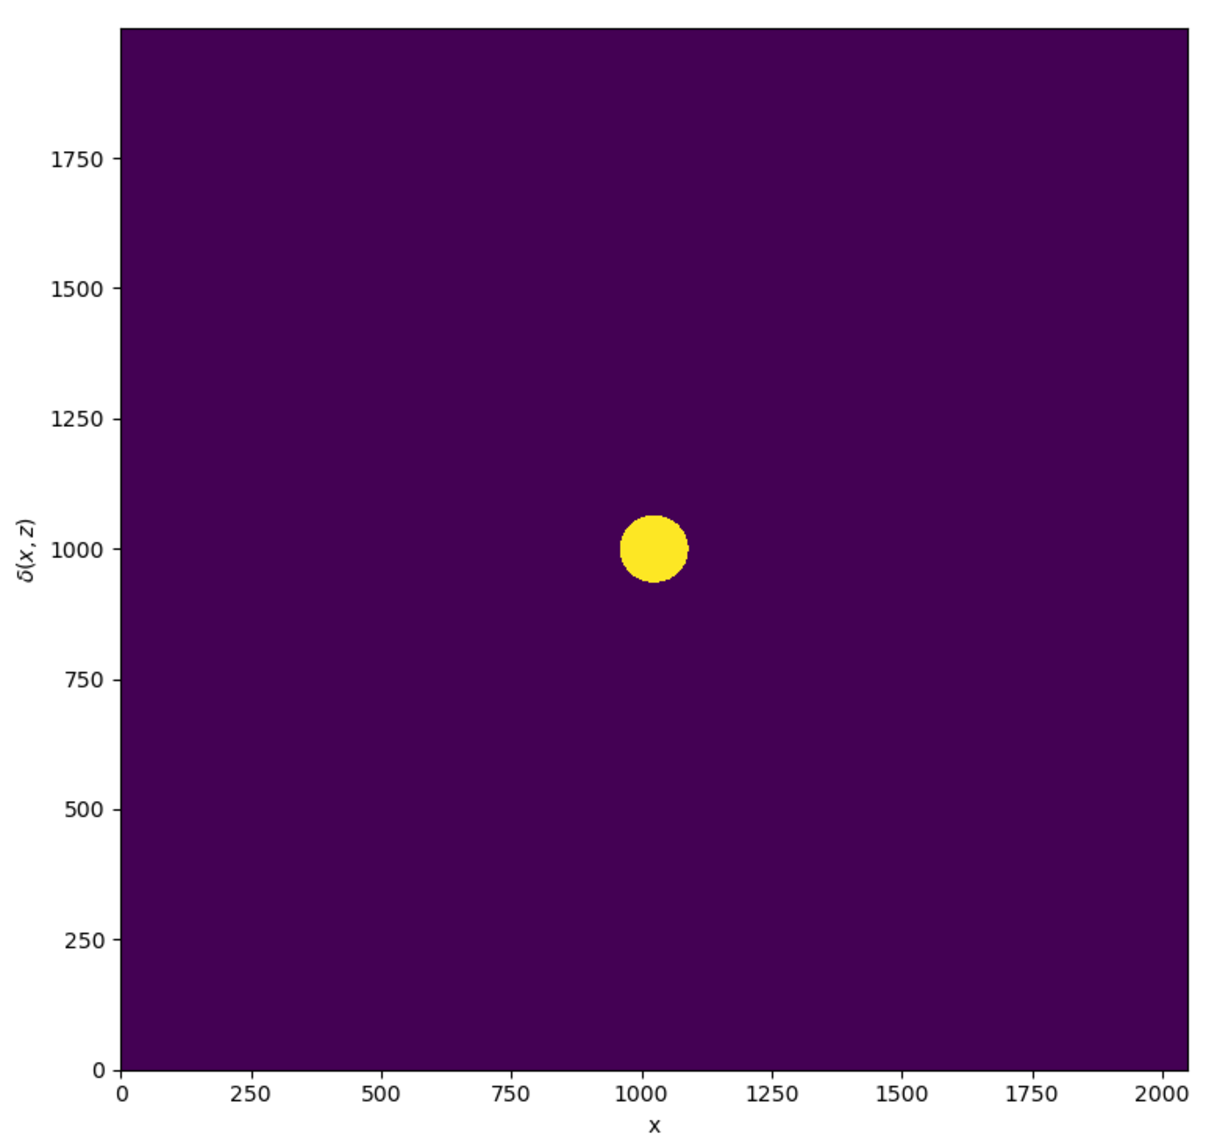
\includegraphics[width=0.6\linewidth]{cross_section.pdf}
% \captionof{figure}{I made this 2D plot to verify that the cross-sectional are a of my simulated cylinder did indeed reflect the correct geometry. Here one can see a purple background representing the complex refractive index value of the vacuum $\delta = 0$ and that of the cylinder in yellow $\delta_0 = 462.8 \times 10^{-9}$ (as was reported in \cite{Beltran} for the PERSPEX sample).}
% \end{Figure}
% \begin{Figure}
% \centering
% 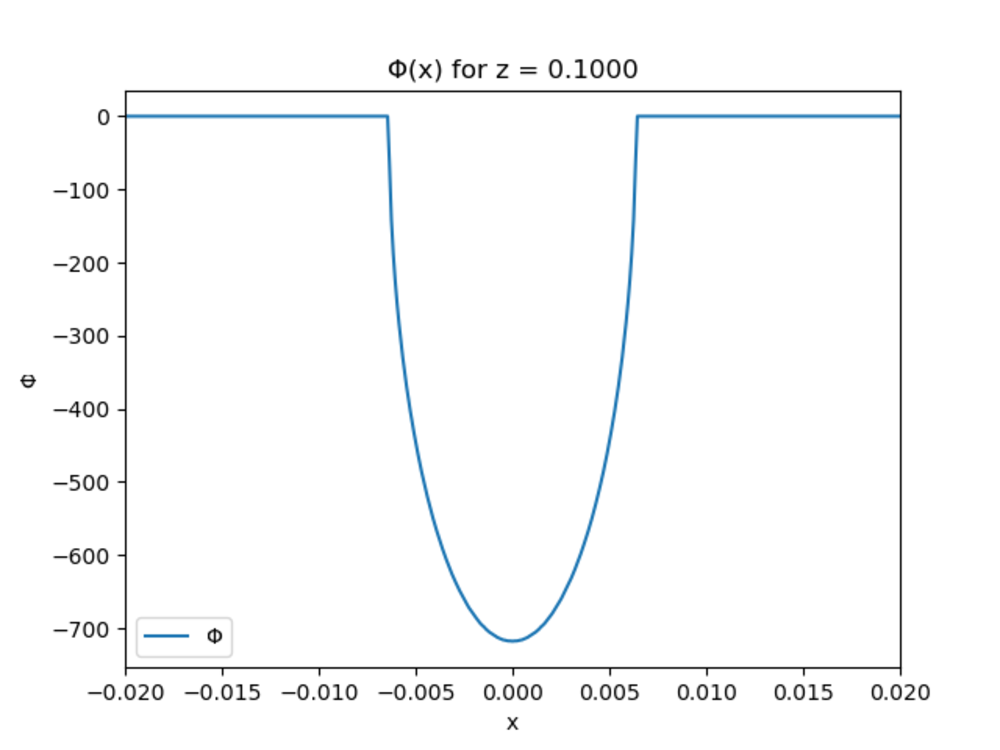
\includegraphics[width=0.6\linewidth]{20000.pdf}
% \captionof{figure}{The position-dependent phase shift I discovered by using fourth order Runge-Kutta.}
% \end{Figure}

\section{Future Plans}
% I aim to finish my simulation by creating a graphic user interface (GUI) that allows the user to modify interactively the density parameters of the imaged concentric cylinders in the simulation. The goal is to make a easily operated visual representation of the changes in phase and intensity of the X-rays as they interact with the object in-situ.

% In the foreseeable future my supervisor and I plan to diversify my project by making me do some simulations about a topic known as speckle analysis. A speckle pattern is commonly produced by interference of coherent light wave-fronts as these transmit through or reflect from a random phase assigning object (scattering medium), the process is known to encode information about the scattering medium that created the speckle\cite{Specks}. The main goal of making me do the speckle simulations is for me to understand the possible sources and causes of speckles in X-ray imaging, and to be able to decode speckle patterns.

% I also plan to aid my supervisor with testing a newly obtained silver target source of X-rays for his lab apparatus. I aim to do data analysis to compare the results from the new silver target to the classic tungsten target used in the apparatus currently.

\section{Conclusion}
% The present aim of my project is to create simulation to investigate how the phase of incident X-rays changes as the density of a sample material in an arbitrary imaging system changes. My investigation will be extended by simulating two distinct materials under the same wave-field and see if and how distinctly phase contrast occurs. The eventual goal of this simulation is to verify if successful phase retrieval can be done of the imaged objects given their variable densities. In this report I present a brief outline of the theoretical perspective of coherent X-ray imaging, a description of my current progress and future aims.

\bibliography{mybib}
\bibliographystyle{unsrt}
\end{document}
